\documentclass{article}

%............Inicia Preambulo.......................
\usepackage{graphicx}
\usepackage{float}
\usepackage[utf8]{inputenc}
\usepackage[shortlabels]{enumitem}
\usepackage{textcomp}
\usepackage{multicol}
\usepackage{caption}
\usepackage[spanish]{babel}
\usepackage[total={17.5cm, 23cm}, top=2cm, left=2cm]{geometry}
\usepackage{esvect}
\usepackage[font=footnotesize]{caption}

\spanishdecimal{.}
\parindent 0cm

%.............Fin de Preambulo........................

\begin{document}

\begin{center}
{\Large \textbf{Universidad Autónoma de Coahuila}}
\end{center}

\begin{center}
{\large Facultad de Ciencias Físico-Matemáticas}
\end{center}

%Materia
\begin{center}
{\large Metodos Numericos}
\end{center}

%Título
\begin{center}
{\large Interpolacion}
\end{center}

%Fecha
\begin{center}
{\large 02 de Diciembre del 2019}
\end{center}

%Autor
\begin{center}
{\large José Antonio Olveda García}
\end{center}

\vspace{5mm}

\begin{multicols}{2}

\section{Objetivo}
\label{sec:obj}
  Explicar y dar introduccion a los metodos de interpolacion comenzando con el metodo simple.

\section{Introduccion}
\label{sec:Int}
La interpolacion consiste en la obtención de nuevos puntos partiendo del conocimiento de un conjunto discreto de puntos.

\section{Metodologia Experimental}
\label{sec:Met}
La interpolación consiste en hallar un dato dentro de un intervalo en el que conocemos los valores en los extremos.
Si se supone que las variaciones son proporcionales se utiliza la interpolación lineal.
Sean dos puntos $(x_{1}, y_{1})$ y  $(x_{3}, y_{3})$, entonces la interpolación lineal consiste en hallar una estimación del valor y, para un valor x tal que $x_{1}<x<x_{3}$.
\begin{figure}[H]
\centering
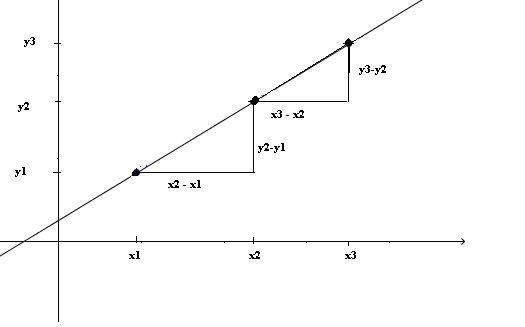
\includegraphics[scale=.5]{Interpolacion.png}
\caption{Interpresentacion de la interpolacion simple}
\end{figure}

Teniendo en cuenta que las variaciones en una relación lineal son constantes entonces podemos determinar por ejemplo las siguientes proporciones:
\begin{equation}
\frac{y_{2}-y_{1}}{x_{2}-x_{1}}=\frac{y_{3}-y_{2}}{x_{3}-x_{2}}
\end{equation}

De igual forma podemos determinar por ejemplo que:

\begin{center}
$\frac{y_{2}-y_{1}}{x_{2}-x_{1}}=\frac{y_{3}-y_{2}}{x_{3}-x_{2}}$
\end{center}

o lo que es equivalente
\begin{center}
$\frac{x_{2}-x_{1}}{x_{3}-x_{1}}$ = $\frac{y_{2}-y_{1}}{y_{3}-y_{1}}$
\end{center}

Despejando $y_{2}$ obtenemos que:
\begin{center}
$y_{2}=y_{1}+\frac{(y_{3}-y_{1})(x_{2}-x_{1})}{(x_{3}-x_{1})}$
\end{center}

\section{Ejemplos}
\label{sec:Ejem}
Si queremos aproximadamente determinar la mediana para el tamaño de las ordenes, a través de interpolación lineal entonces podemos proceder de la siguiente manera:
\\
\\
\begin{tabular}{|l|l|l|l|}
\hline
Tamaño de & No. de ordenes & Por. de ordenes & Porc. acum. \\
\hline
[0,10) & 950 & 23.3 & 23.3 \\
\hline
[10,25) & 940 & 23.1 & 46.4 \\
\hline
[25,50) & 110 & 2.7 & 49.1 \\
\hline
[50,100) & 680 & 16.7 & 65.8\\
\hline
[100,250) & 260 & 6.4 & 72.2\\
\hline
[250,500) & 480 & 11.8 & 84 \\
\hline
[500,1000) & 650 & 16 & 100 \\
\hline
\end{tabular}
\\
\\
\\
Observando la tabla de distribución de frecuencias vemos que el intervalo que acumula el 50 porciento de los datos es $[50,100)$, por lo tanto en él está contenida la mediana.
Ahora suponiendo que las frecuencias están distribuidas proporcionalmente en el intervalo:

$50-----------49,1$
\\
$Me-----------50$
\\
$100-----------65,8$
\\
\\
podemos plantear por ejemplo la siguiente proporción:

\begin{center}
$\frac{Me-50}{100-50}= \frac{50-49.1}{65.8-49.1}$
\end{center}

Despejando

\begin{center}
$Me=50+ \frac{(100-50)(50-49.1)}{65.8-49.1}$ = 52.99
\end{center}

La interpolación se puede realizar tanto con las frecuencias acumuladas absolutas, como con las relativas o relativas porcentuales.

\section{Ventajas y Desventajas}
\label{sec:Ven}
\textbf{Ventajas}
\\
1. La interpolacion lineal es rapida y facil, ya que solamente se hace el calculo de trayectoria de dos puntos.
\\
2. A pesar que se puede producir errores de calculo entre intervalos, existe la funcion de error que se puede aproximar "x"
a "$x_{n}$", a que representaria el punto medio entre los dos puntos.
\\
3. Entre mas pequeño sea el intervalo entre dos puntos, mas exacta sera la aproximacion.
\\
\\
\textbf{Desventajas}
\\
1.A pesar de ser rapida y sencilla, no es muy precisa.
\\
2. Si el comportamiento no corresponden al de una recta los valores calculados no son correctos.
\\
3. Por interconectar dos puntos en una linea recta de un polinomio los resultados no se ajustan con exactitud para calcular el punto medio entre los mismo por ello es mas efectivo el metodo cuadratico 
\section{Implemetacion del programa}
\label{sec:res}
\begin{figure}[H]
\centering
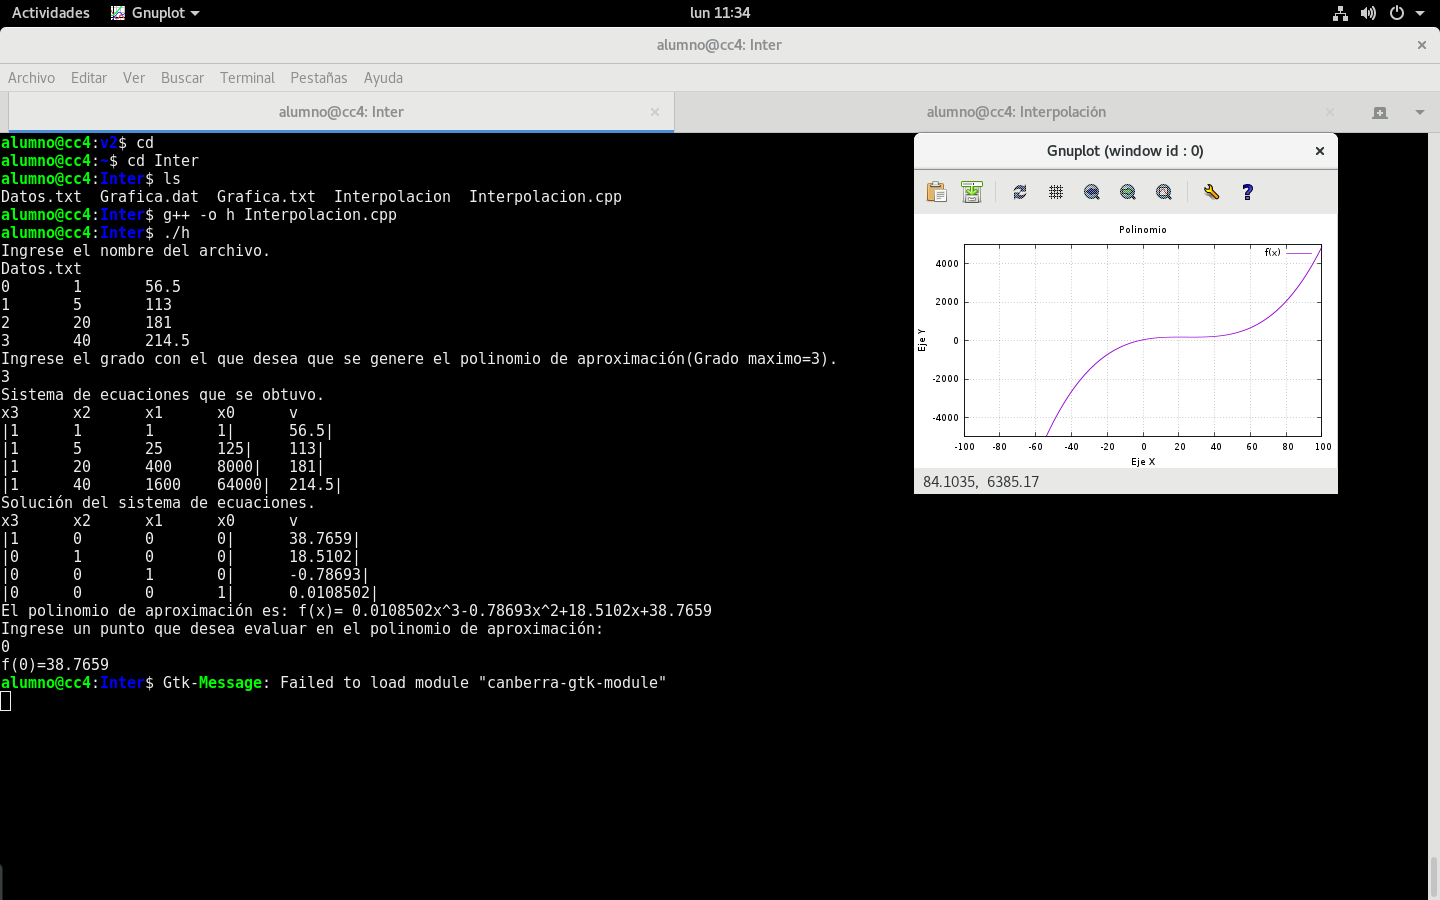
\includegraphics[scale=.125]{Interpolacion2.png}
\caption{Ejemplo de Interpolacion aplicado al programa}
\end{figure}
Como podemos apreciar en la figura anterior, los datos de interpolacion dados, se guardan en un archivo llamado "Datos.txt", esto para evitar tener que estar ingresando los datos cada vez que se tenga que hacer la ejecucion del programa, Obteniendo el sistema de ecuaciones otorgado, y segun la cantidad de datos del sistema es como se obtendra el polinomio de interpolacion dado, en este caso su grado maximo sera de 4, como se observa en la figura.
\section{Conclusión}
\label{sec:concl}
El metodo de interpolacion simple es muy facil y rapido, sin embargo las graficaciones y aproximaciones generadas sobre esta no son precisas del todo, obteniendo errores grandes en su ejecucion

\end{multicols}

\end{document}
